\section{Project Management} \label{sec:pm}
\todo[inline, color=yellow]{Vera}

This chapter describes the project planning and management of the \textit{Interaction Lab}. It is divided into the different project phases. Each division includes all important facts of its project period.

\subsection{Project Definition} \label{sec:PMProjectdefinition}
\todo[inline, color=yellow]{Vera}
This section describes the results of the project definition phase in detail. This includes a problem analysis, a list of objectives and requirements, a solution concept as well as a workability analysis.

\subsubsection{Problem Analysis}\label{sec:PMProblemAnalysis}
\todo[inline, color=yellow]{Vera}
The demand for Virtual Reality (VR) devices and applications increased heavily since the first consumer devices like \textit{HTC Vive} and \textit{Oculus Rift} were released during last years. One main difficulty of the current development of VR-applications is the lack of standardisation of the Software Development Kit (SDK) and interfaces. The most acknowledged suppliers \textit{HTC} and \textit{Oculus} do not work together or force standards for VR application development. Thus, all applications are system related and incompatible with other devices. Accordingly, each device offers different opportunities of interaction methods. These methods could be divided in the acknowledged categories selecting, grabbing, manipulating, movement and indirect controlling via widgets, gestures and voice input. Several suppliers currently offer different devices for interaction. And with focus on the grabbing and positioning methods, the most common are the \textit{Oculus}-HMD, \textit{HTC Vive}-HMD, \textit{HTC Vive}-Controller, data gloves and motion capturing systems for hand-tracking like the \textit{LeapMotion}-Controller.

As mentioned in section \ref{sec:Motivation}, there exist currently no interaction laboratory which compares the different interaction methods in a scientific and credible way. Hence, the development of a virtual laboratory is highly requested to compare and test different interaction methods in adequate test environments. Thus, user friendly interaction methods which nearly full-fill usability requirements could be improved by researcher which yields to a higher demand of VR devices and application. That will squeeze the profit of VR device suppliers which include those user friendly interaction methods. 

\subsubsection{Usage Context}\label{sec:PMUsageContext} 
\todo[inline, color=yellow]{Vera}
Hence, the required laboratory has mainly two usage contexts. First, it could be used to run scientific studies in VR research or development. Second, it could demonstrate and exemplify the differences of grabbing interactions in education proposes or support the students to develop and test grabbing methods on their own during lectures. 

\subsubsection{Objective and Requirements}\label{sec:PMRequirements}
\todo[inline, color=yellow]{Vera}

At least two scenes should be realised to provide a laboratory which allows to run scientific and reliable study as well as is useful for the education of students. In the first scene, the user will be able to learn the offered grabbing methods. Therefore, this room is will provide simple cubes of various sizes which are in different distances from the users. Every cube is moveable and could be placed at every place. Each user is forced to follow the introductions of a self teaching before every offered method could be tested independently. The current user can only begin with the actual study after every method is trained to ensure equal preconditions.

The second room will be modelled after a supermarket because this model offers various options of grabbing and positioning tasks. In this room, the participant will get different tasks which will differ by complexity, distance of grabbing and size of the objects. The user will be able to change the options of grabbing independently but not choose the current method. An optional extension of the project will be another type of task where the user decides which type of method is preferred for this task.

The grabbing methods can be categorised into close range and far range and include the grabbing, rotating, and positioning of an object. Possible types of close range methods, are the actual touching of a movable object to select it or by holding the controller in the proximity of it but without touching it. Another more precise option is the selection with a thin wand in front of the controller. This of collection of methods that includes close human cognition methods as well as less or very accurate ones. 
The far range interaction will have different options as well. One will be a ray that shoot out of the controller, another one will extend a ray from the head and the third one will extend the arm in the pointed direction. This means the user will be able to point at an object with the controller or to look in the direction of it.

The system offers two measurements and the related saving of the different parameters. First, the duration time is measured for every performed task to compare and validate the performance of the different interaction methods. Second, every single grabbing try of a task will be counted and saved to get a conclusion about the learn-ability, accuracy, and performance.

Furthermore, there will be a questionnaire designed to give the users of \textit{Interaction Lab} an usability evaluation tool at hand. This questionnaire will test parameters as tiring, learnability, self-descriptiveness and fulfilling expectations.


\subsubsection{Solution Concept}\label{sec:Projectconcept}
\todo[inline, color=yellow]{Vera}
An interaction laboratory for grabbing and positioning interactions at close or far range will be developed in \textit{Unity}. It includes two test rooms e.g. scenes, where the first is a learning room, in which the users can get familiar with the interaction methods. The second room is designed as a supermarket. This environment was chosen because it offers various possibilities of exercises under changing difficulties like grabbing small mushrooms, fetching distantly placed tins or putting goods on provided target areas. The exercises are offered in form of a tasks that tells the participant what goods have to be grabbed and repositioned. These various tasks are predefined and cover all difficulties that a type of grabbing method could have. They are displayed on tables which are connected to the controller and could be shown or hide in the controller menu. 

All rooms are implemented in Unity and the VR components are controlled by the same framework. Further, the \textit{HTC Vive}-HMD and the corresponding controllers are used to run the interactions, imaging and orientation in the environment. It is planned to realise at least six interaction methods of grabbing and positioning. Additional, the complete framework should be compatible with new test scenes and other interaction categories. 

The system offers a measurement of the accuracy as well. A time measuring of duration and an error rate for every performed task is planned. Each measuring of every room is automatically saved in an output file which could be easily imported in common statistic tools. Furthermore, there will be a validated questionnaire designed to give the users a usability and simulator sickness evaluation tool at hand. This usability questionnaire will test parameters as tiring, learn-ability, self-descriptiveness and fulfilling expectations of each method. Whereas the simulator sickness evaluation asks for motion sickness and other system properties of the complete system. All questionnaires are validated and fit the requirement of VR systems and application. The results of each questionnaire will be saved in an output file as well.

\subsubsection{Workability Analysis}\label{sec:PMworkabilityAnalysis}
\todo[inline, color=yellow]{Vera}
There are several risks according to the concept in section \ref{sec:Projectconcept}. First, the measurements could be implemented incompletely or inaccurately. This can be avoided by a thorough testing before the final release with some external test persons. The tasks could be incomprehensible for them as well which should be prove as well.
The system integration future extensions could cause trouble. Therefore, the systems architecture should be designed wisely and consequently to avoid incompatibilities. Another risk of the implementation is that they might be more costly and complex as recommended but this is widely acknowledged. After the implementation is finished the interaction method performance or validation could be too expensive which results in a higher latency. These circumstances must be observed during the implementation and testing. Due to the high workload of the testing, the time slot for it and the trouble shooting might be underestimated. Another time risk is that there is limited access to the facilities and VR laboratory because of the huge number of running project at the current time.

Nevertheless, the concept is feasible and the project goals could be achieved during the time schedule because all the risk seems to manageable and could be observed during the scheduled testing.

The demand of the students project are satisfied and a financial profitability check is not necessaries due to the fact that the facilities of the university can be used and no further purchases are affordable.


\subsubsection{Project Organisation}\label{sec:PMProjectOrganisation}
\todo[inline, color=yellow]{Vera}

The project manager is Vera Brockmeyer who mainly should manage the appointments and facilities as well as to communicate to the outside. The latter is done via email or in a meeting with the concerned persons. Another task is to create and maintain the project plans that includes to keep the overview of the complete project progress and to ensure the milestones.
The current state should be hand out weekly to the team in form of an email or a team meeting.

All other team members have their own responsibilities. Anna is head of the scene building which includes the definition of the general scene design, research, and to inform the project manager about current problems and timing. The latter two points concern each head of a section. The other section is split into the close and far range interactions. The head of close range interaction is Britta Boerner and the other is Laura Anger. Both manage the implementation of their section.

The formal an informal non-verbal communication in the team is done via email with the subject \textit{VR Interface Lab} and a \textit{Google Calendar} is exclusively maintained by the project manager where all team appointments are intercalated. This calendar shows the availability of all team members and the VR laboratory, too. More complex problems or team decisions are made in the weekly team meeting with stringently required appearance. Due to the requirements and availability of the team members, the meeting is held via \textit{Skype} or in personal.

All files belonging to the project are organized in a cloud folder of \textit{Google Drive} or in two \textit{GitHub} repositories. The first one is for all \textit{LaTex} files and the second manage the complete framework. Whereas the cloud folder contains presentation files, graphics and images, To-Do-List, papers and more.

The required facility is one of the VR laboratory of the faculty which should have a minimum size of $15$qm and be located in the university building. These laboratories have a complete \textit{HTC Vive}
system and a compatible computer (see Table \ref{tab:Computer}).

\subsection{Project Planning} \label{sec:PMProjectPlanning}
\todo[inline, color=yellow]{Vera}
This section list all required projects plans like a work breakdown structure, the work packages, a capacity and cost plan as well as a quality plan.
\subsubsection{Work Breakdown Structure}\label{sec:PMWBS}
\todo[inline, color=yellow]{Vera}
The work breakdown structure (see Figure \ref{fig:wbs}) is split in four groups. First, the project planning which contains the actual project management as well as the research work packages Second, the implementation group includes the development of the laboratory environment and the six interaction methods. Third, the evaluation contains the work packages of tasks including measurements and the questionnaires. Finally, the last group includes the documentation and project profile packages.

\begin{figure}[H] 
	\center 
	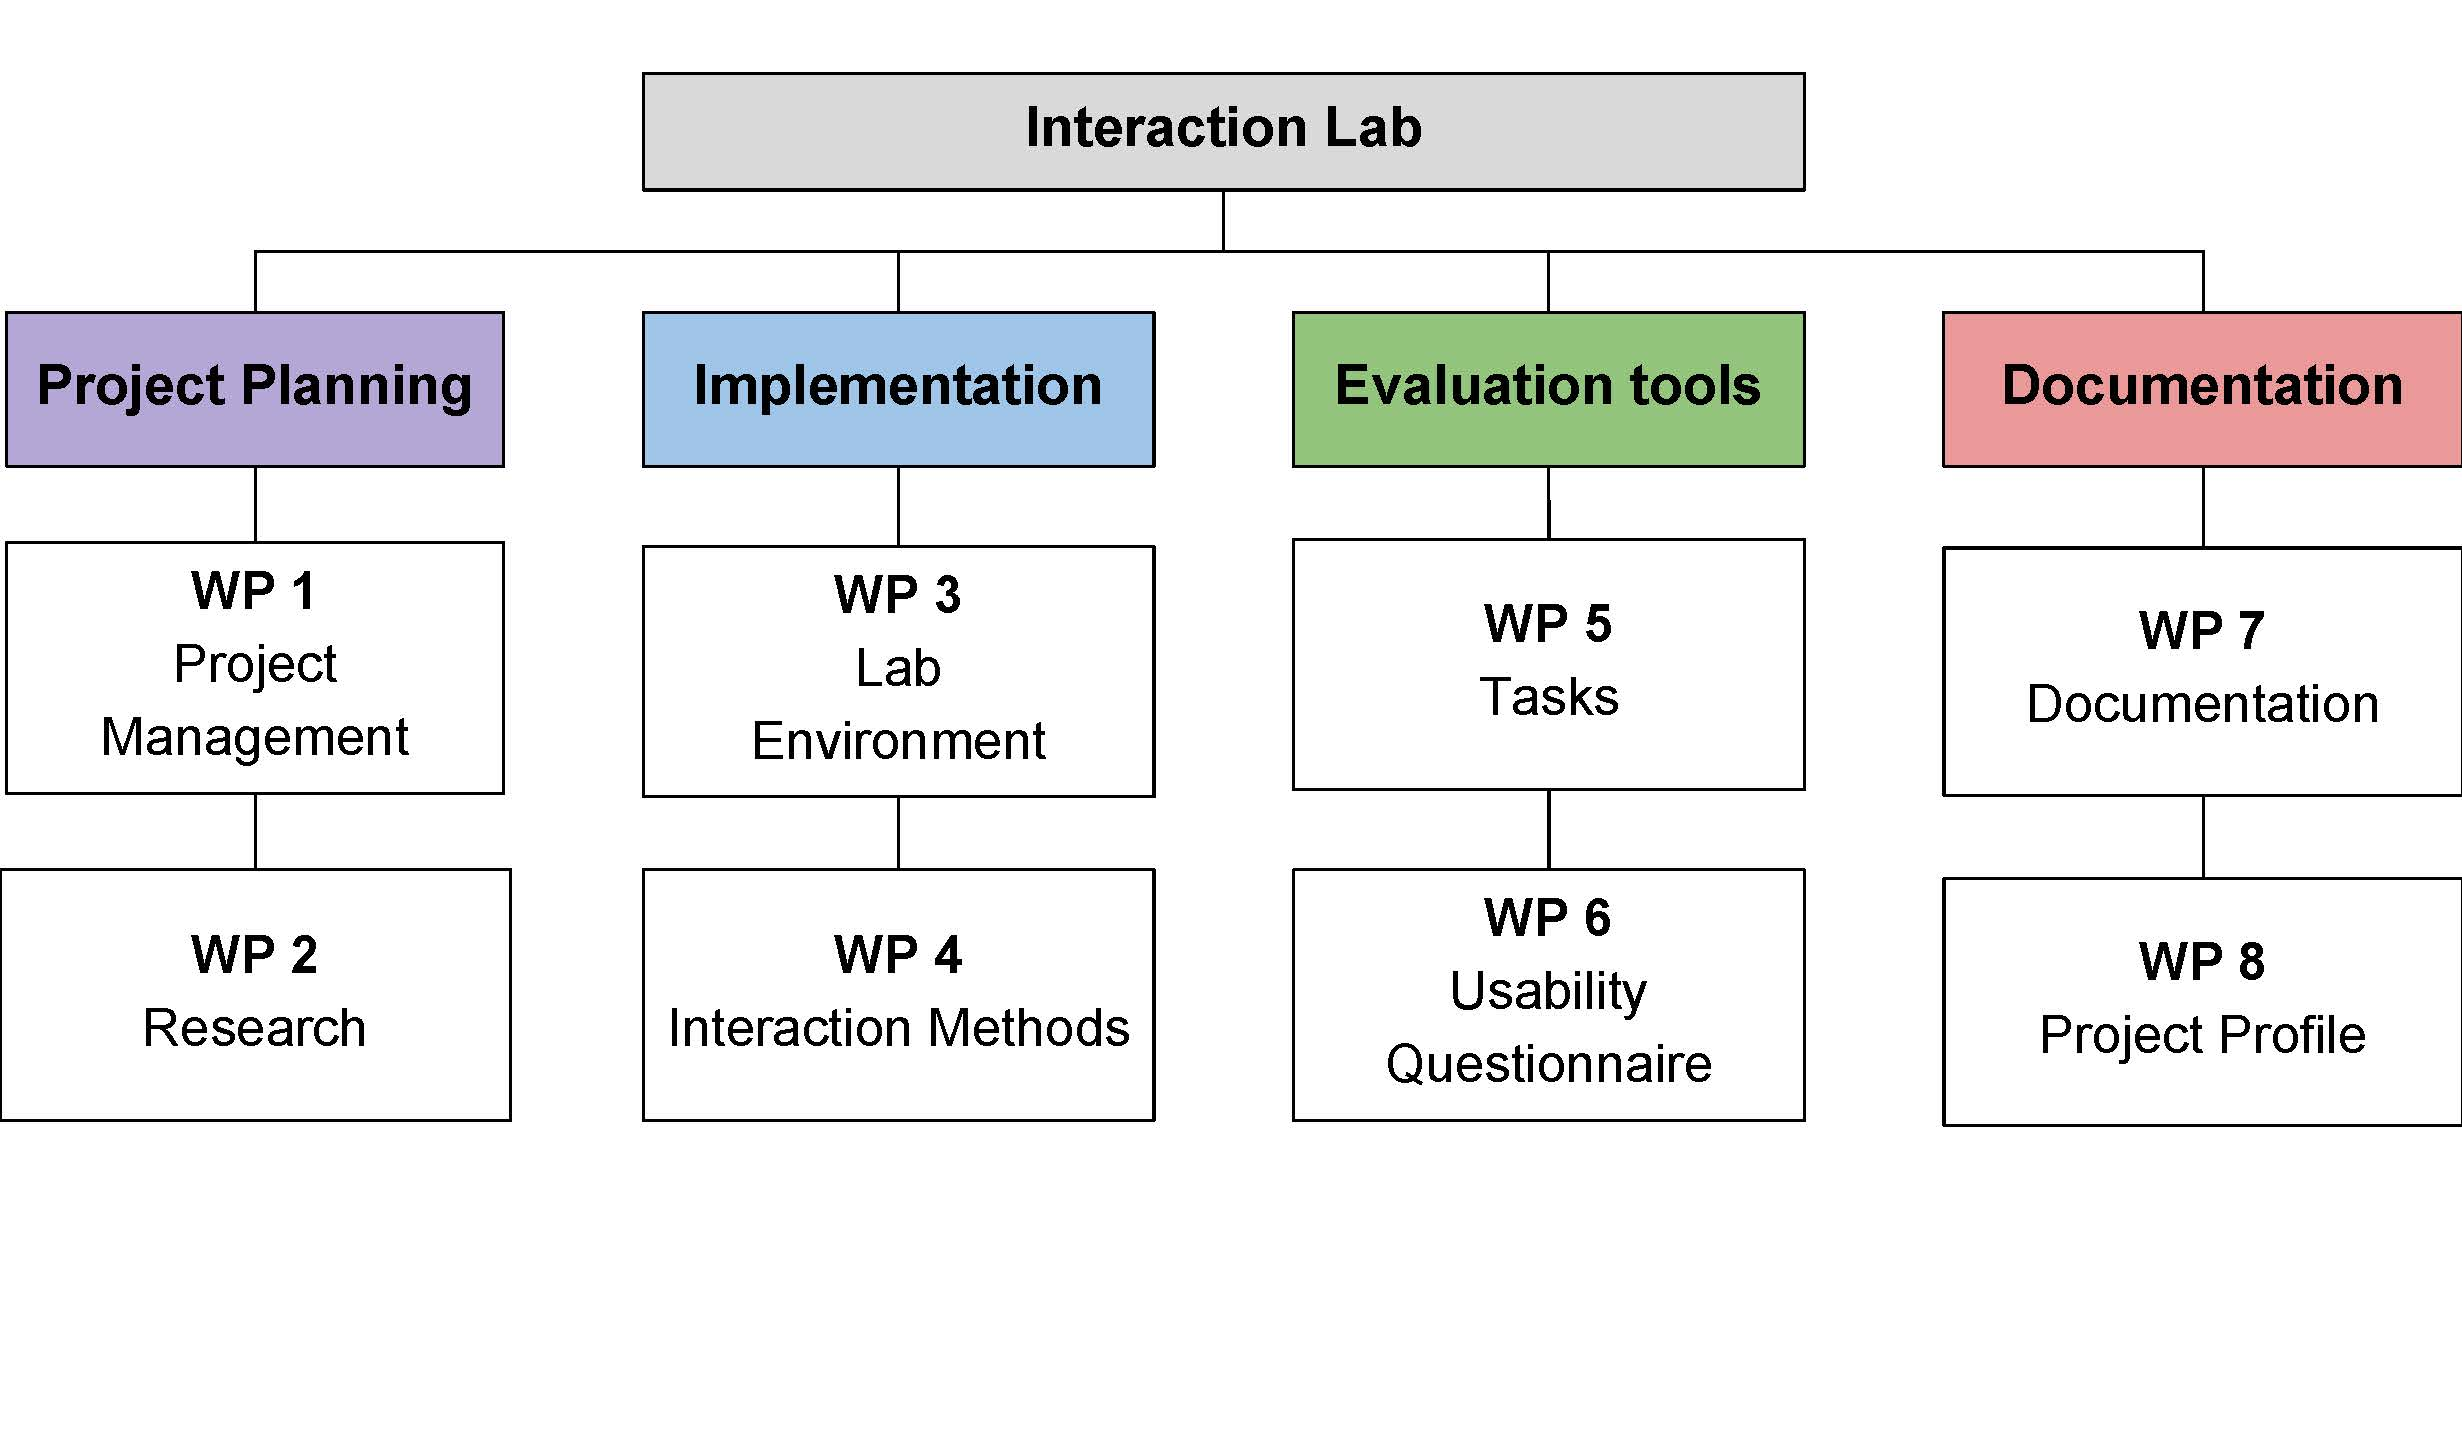
\includegraphics[width= 15 cm]{Images/WBS.jpg}			
	\caption[]{Work Breakdown Structure}
	\label{fig:wbs}
\end{figure}
\subsubsection{Workpackages}\label{sec:PMWorkpackages}
\todo[inline, color=yellow]{Vera}
A complete listing of the work packages according to Figure \ref{fig:wbs} could be seen in the Appendix A \ref{sec:AppendixA}.

\subsubsection{Project Schedule}\label{sec:PMSchedule}
\todo[inline, color=yellow]{Vera}

Figure \ref{fig:wbs} shows the project schedule with the timing of all work packages. The most important deadlines are the project plan, research, first and second prototype as well as the release deadline. First, the project plan should be finished until 13th April 2017. Second, the research deadline is two and a half weeks later at the 27th April 2017. Followed by both prototypes which are set for the 31st may and 30th June 2017. The final release deadline is at the 15th July 2017.

\begin{figure}[H] 
	\center 
	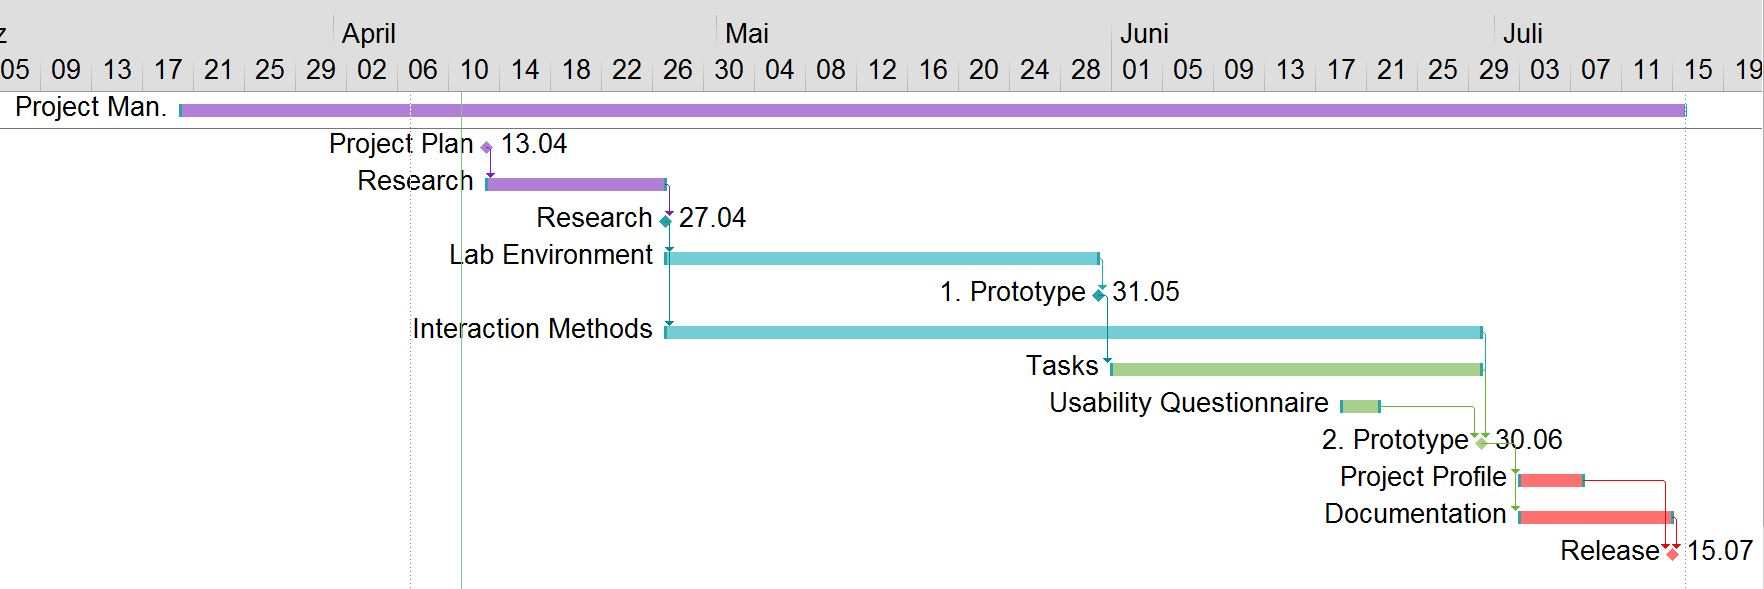
\includegraphics[width= 15 cm]{Images/Gantdiagramm.jpg}			
	\caption[]{Project Schedule}
	\label{fig:wbs}
\end{figure}

\subsubsection{Capacity Plan}\label{sec:PMCapacity Plan}
\todo[inline, color=yellow]{Vera}

The capacity plan lists the estimated time resources of each team member, the availability of the required laboratory with the \textit{HTC Vive} system and the SLR camera for the documentation.
\begin{table}[H]
	\centering
	\begin{tabular}{|l|l|l|l|}
		\hline
		\Absatzbox{}
		\textbf{Resource} &	\textbf{ Estimated [h]} &	\textbf{Actual [h]} & 	\textbf{Buffer [$\%$]}\\ \hline
		Laura &	166 &	180	& 7.78\\ \hline
		Anna&	170	&180&	5.56\\ \hline
		Vera&	182	&180&	-1.11\\ \hline
		Britta&	168&	180	&6.67\\ \hline
		Total Personal&	686	&720&	4.72\\ \hline
		VR Lab 1&	173&	152&	-13.82\\ \hline
		SLR Video Camera&	8&	8&	0.00\\ \hline
	\end{tabular}
	\caption[]{Capacity Plan of personal and facility resources.}
	\label{tab:Capacity Plan}
\end{table}

\subsubsection{Cost Plans}\label{sec:PMCostPlan}
\todo[inline, color=yellow]{Vera}

The cost plan of personal resources in Table \ref{tab:Personal Cost Plan} gives a more detailed overview of the estimated time resources per work package. It is structured into the cost of each team member and the total cost of a work package. Whereas, the cost plan of the facility resources offers an overview of the material costs and their providers.

\begin{table}[H]
	\centering
	\begin{tabular}{|p{5cm}|p{1.5 cm}|p{1 cm}|p{1cm}|p{1.5 cm}|p{2 cm}| l l l l l l }
		\hline
		\Absatzbox{}
	\textbf{Name}&	\textbf{Laura [h]} &\textbf{Anna [h]} &	\textbf{Vera [h]} &\textbf{	Britta [h]} &	\textbf{Cost WP [h]} \\ \hline
	Project Management &	12&	12&	45&	12&	81\\ \hline
	Research&	10	&10	&10&	10	&40\\ \hline
	Lab Environment&	0&	55&	32	&10&	97\\ \hline
	Interaction Methods	&65&	0&	0&	65	&130\\ \hline
	Tasks	&15&	45	&30&	15&	105\\ \hline
	Usability Questionnaire	&8	0&	0&	0&	8\\ \hline
	Documentation	&45	&45&	55&	45&	190\\ \hline
	Project Profile	&8	0&	0&	8&	16\\ \hline
	\textbf{Total Cost}	&\textbf{163}&	\textbf{167}	&\textbf{172}&	\textbf{165}	&\textbf{667}\\ \hline
	
	\end{tabular}
	\caption[]{Cost Plan of personal resources.}
	\label{tab:Personal Cost Plan}
\end{table}

\begin{table}[H]
	\centering
	\begin{tabular}{|p{3cm}|p{1 cm}|p{1.5 cm}|p{1.5cm}|p{1.5 cm}|p{3.5 cm}| l l l l l l }
		\hline
		\Absatzbox{}
		\textbf{Ressourcen}	&\textbf{Quan- tity}&	\textbf{Unit Price [EUR]}&	\textbf{Cost [EUR]}&\textbf{Act. Cost [EUR]}&\textbf{Comments} \\ \hline
			 HTV Vive &	1	&899&	899&	0	&Price of Vive Online Shop, provided by TH Cologne\\ \hline
			 SLR Camera&	1	&500&	500&	0	&estimated, provided by team member\\ \hline
			 VR Computer&	1	&1800&	1800	&0	&offer from Computer Shop, provided by TH Cologne\\ \hline
			 MS Office	&1	&149&	149&	0&	provided by TH Cologne\\ \hline
			MS Project&	1	&195&	195&	0&	provided by TH Cologne\\ \hline
			3D assets of Food Beverages&	2&	15&	30&	0	&Steam\\ \hline
	\textbf{Total}	&	& &	\textbf{3573}	&\textbf{0}	&\\ \hline
		
	
	\end{tabular}
	\caption[]{Cost Plan of facility resources.}
	\label{tab:facility Cost Plan}
\end{table}


\subsubsection{Quality Plan}\label{sec:PMQualityPlan}
\todo[inline, color=yellow]{Vera}
\begin{table}[H]
	\centering
	\begin{tabular}{|p{3cm}|p{3 cm}|p{3.5 cm}|p{3.5cm}|}
		\hline
		\Absatzbox{}
		\textbf{Quality Goal}&	\textbf{Criteria} &\textbf{Method} &	\textbf{Controlling}\\ \hline
	Immersion and Presence	& no distraction by real world &	Presence questionnaire by Witmer and Singer; questions according to sound and haptic will left out	& use and evaluate brief questionnaire during functionality test\\ \hline	
Low Latency	& under $20$ms &	keep the scenes as simple as possible & show the frames per second in the Unity console\\ \hline		
No dropouts	& no black frames or errors in the unity project & no expensive or parallel calculation & visual testing\\ \hline	
Understandability of tasks	& correct task performance by test user during functionality tests & use common objects and tasks; brief and precise task descriptions & use brief questionnaire during functionality test\\ \hline	
robust system & Vive System does not crash during process & no expensive calculations; control and calibration of hardware; analyse and solve directly problems & observe during development
\\ \hline
Correct saving of Usability Questionnaire Response & entire answers of study participants are correctly saved in an file & Use of Google Forms & functionality test and controlling of completeness and correctness\\ \hline
Understandability of Usability Questionnaire & no questions or uncertainties of test users& validated Usability Questionnaire & use and evaluate brief questionnaire during functionality test\\ \hline
	\end{tabular}
	\caption[]{Quality Plan}
	\label{tab:Qaulity Plan}
\end{table}
\subsection{Project Execution} \label{sec:ProjectExecution}
\todo[inline, color=yellow]{Vera}
The following sections summarizes the project progress as well as the problems that caused a delay of the schedule.
\subsubsection{Project Progress}

In general, the project progress went off quite well and most of the project goals were achieved and are running as expected. Therefore, the \textit{Interaction Lab} is a complete and running application that includes all required tools for a scientific study. The final system contains a learning room, a supermarket test scene with implemented task and measuring, the implementation of five different interaction methods to test, completely set of validated usability questionnaires and excel templates for the evaluations.

However, some of the project goals were too ambitious for the resources capacity in the scheduled time window. Thus, not all project goals were completely achieved. First, the Gogo interaction method and the HMD raycast could not be developed due to the problems mentioned in section \ref{sec:PMProblems}. Second, the number of tasks needed to be reduced significantly because it turned out that they are too time consuming during testing. Hence, only one task was implemented with all provided interaction methods and three tasks to figure out the preferences of the users for various kind of ranges and object sizes. Third, an additional goal was set after the first prototype. A self teaching mode has been added to the learning room to ensure an equal introduction of the methods and task for each test user.

The actual workload of most work packages covers their estimation beside some problems which are described in detail in section \ref{sec:PMProblems}. All team members had a similar work load and the task allocation work efficient and well. Each team member knew their current tasks at every time and had an overview of the complete progress. This overview was achieved with weekly meetings via \textit{Skype} or if affordable in personal. Furthermore, every few weeks we had a meeting with Prof. Grünvogel to give him an update and discuss current problems and their solution.


\subsubsection{Problems and Solutions}\label{sec:PMProblems}
\todo[inline, color=yellow]{Vera}

A first problem was the additional work effort because all project plans needed to be overworked which causes a one week delay. In the end, it should also be noted the planning was to detailed in the beginning which cause some unnecessary time. Thus, the research phase need to shorten and place on hold for this week but this step brought the project back on time. Another delay of one and a half week causes the inevitable unity and \textit{HTC Vive} system that were more difficult than expected. This kind of problem occurs several times when changing the laboratory due to limited capacities of the designated VR Lab 1 or the periphery of the laboratories were not present. Additional, every time the VR systems needs to be recalibrated when changing the laboratory.

The VR system causes trouble during the implementation of the HMD Raycast method, too. It turned out that the tracking of the HMD lacks precision and the ray drifts at the border of the view field. At this point, the number of tasks that must be done to guarantee a working application until the release was challenging. Thus, we concentrate on a working application and discard the HMD Raycast. However, it seems that the implementation of the Gogo method was too complex for this time schedule, too. Hence, it was changed to the Extenable Ray method which could be implemented successfully during the calculated period. 

This decision and the resulting choice of methods had the advantage that their basic structure is adoptable. Regarding to this realisation, it could be said that the split of responsibility for Far and Close Range in the project organisation was a mistake. Accompanied with the decision to create a single C\# script per method. This plenty of scripts caused a lot of trouble during their integration in the final application but these problems were solving by using only one script for similar methods like the ray methods, for example.

\newpage

























